\section{Simulation Results}
\label{chap:results}
\subsection{Instrument-Relevance Calibration}
\label{sec:results-relevance-calibration}

Table~\ref{tab:strength-calibration} checks whether the four values of $\kappa$ produce the intended ordering of excluded-instrument relevance. In each calibration replication, the restricted OLS regression uses the continuous treatment $D$ as the dependent variable and includes an intercept and $X_1,\ldots,X_{10}$. The unrestricted regression adds $Z_1$ and $Z_2$, which are tested jointly. The reported nested-regression $F$-statistic and partial $R^2$ are calculated over 100 replications for every $(n,\kappa)$ design. They are descriptive first-stage diagnostics rather than formal IVQR identification statistics.

\begin{table}[!htbp]
  \caption{Instrument-strength calibration}
  \label{tab:strength-calibration}
  \begin{booktabs}{
    colspec = {Q[c] Q[c] Q[r] Q[c] Q[r] Q[c]},
    row{1} = {font = \bfseries}
  }
$n$ & $\kappa$ & Median $F$ & $F$: p10--p90 & Median partial $R^2$ & Partial $R^2$: p10--p90 \\
500 & 1.00 & 101.17 & 85.93--126.68 & 0.294 & 0.261--0.342 \\
500 & 0.50 & 18.71 & 11.99--27.95 & 0.071 & 0.047--0.103 \\
500 & 0.25 & 4.74 & 1.74--8.65 & 0.019 & 0.007--0.034 \\
500 & 0.10 & 1.22 & 0.24--3.65 & 0.005 & 0.001--0.015 \\
1000 & 1.00 & 212.82 & 185.34--239.50 & 0.301 & 0.273--0.327 \\
1000 & 0.50 & 38.65 & 30.13--53.60 & 0.073 & 0.058--0.098 \\
1000 & 0.25 & 9.85 & 5.34--16.15 & 0.020 & 0.011--0.032 \\
1000 & 0.10 & 2.04 & 0.38--5.42 & 0.004 & 0.001--0.011 \\
  \end{booktabs}
  \begin{tablenotes}[Note]
    Descriptive Monte Carlo instrument-relevance diagnostics. The reported dispersion ranges are the 10th and 90th percentiles.
  \end{tablenotes}
\end{table}


Both diagnostics decrease at every step as $\kappa$ falls. For $n=500$, the median $F$-statistic declines from $101.17$ at $\kappa=1$ to $18.71$, $4.74$, and $1.22$ at the three weaker settings. For $n=1000$, the corresponding sequence is $212.82$, $38.65$, $9.85$, and $2.04$. The dispersion ranges in Table~\ref{tab:strength-calibration} shift in the same direction. Median partial $R^2$ falls from $0.294$ to $0.005$ for $n=500$ and from $0.301$ to $0.004$ for $n=1000$, with intermediate values near $0.07$ at $\kappa=0.50$ and $0.02$ at $\kappa=0.25$.

At a fixed $\kappa$, partial $R^2$ is similar across the two sample sizes because it records the incremental explanatory share of the two instruments. The $F$-statistic nevertheless rises with $n$ because that contribution is estimated more precisely with more observations. The joint movement of the two diagnostics therefore confirms the designed relevance ordering: $\kappa=1$ provides the strongest relationship and $\kappa=0.10$ the weakest. This ordering is used to organise the results below; it does not impose a conventional first-stage threshold or establish a universal IVQR identification classification.

\subsection{Point-Estimation Accuracy}
\label{sec:results-point-accuracy}

Table~\ref{tab:main-performance} displays finite-sample performance for $n=1000$, the representative quantiles $\tau\in\{0.10,0.50,0.90\}$, all four $\kappa$ values, and the three estimators. The comparisons in this subsection also use the complete saved results for both sample sizes and all five quantiles. Each point estimate is the first minimiser of the candidate-specific statistic on the ordered 41-point grid in $A_0=[-1,3]$, rather than a continuously optimised estimate.

\begin{table}[p]
  \small
  \caption{Main finite-sample performance at $n=1000$}
  \label{tab:main-performance}
  \begin{booktabs}{
    colspec = {Q[c] Q[c] X[l] Q[r] Q[r] Q[r] Q[r] Q[r]},
    colsep = 2pt,
    rowsep = 0pt,
    row{1} = {font = \bfseries},
    hline{14,26} = {\lightrulewidth, solid}
  }
$\tau$ & $\kappa$ & Estimator & Bias & MAE & RMSE & Coverage & {Median\\accepted-set\\measure} \\
\SetCell[r=12]{c} 0.10 & \SetCell[r=3]{c} 1.00 & Oracle-GMM & -0.054 & 0.093 & 0.121 & 0.860 & 0.400 \\
 &  & Full-GMM & -0.329 & 0.337 & 0.387 & 0.502 & 0.800 \\
 &  & DML-IVQR & -0.005 & 0.117 & 0.150 & 0.968 & 0.600 \\
 & \SetCell[r=3]{c} 0.50 & Oracle-GMM & -0.101 & 0.194 & 0.287 & 0.926 & 1.000 \\
 &  & Full-GMM & -0.407 & 0.465 & 0.630 & 0.804 & 1.900 \\
 &  & DML-IVQR & -0.159 & 0.306 & 0.482 & 0.948 & 2.225 \\
 & \SetCell[r=3]{c} 0.25 & Oracle-GMM & -0.384 & 0.566 & 0.934 & 0.930 & 3.450 \\
 &  & Full-GMM & -0.773 & 0.914 & 1.242 & 0.932 & 3.500 \\
 &  & DML-IVQR & -0.681 & 0.844 & 1.229 & 0.950 & 3.750 \\
 & \SetCell[r=3]{c} 0.10 & Oracle-GMM & -0.747 & 0.975 & 1.376 & 0.946 & 4.000 \\
 &  & Full-GMM & -1.074 & 1.251 & 1.582 & 0.942 & 3.900 \\
 &  & DML-IVQR & -0.932 & 1.146 & 1.514 & 0.936 & 4.000 \\
\SetCell[r=12]{c} 0.50 & \SetCell[r=3]{c} 1.00 & Oracle-GMM & 0.007 & 0.047 & 0.072 & 0.872 & 0.200 \\
 &  & Full-GMM & 0.007 & 0.072 & 0.100 & 0.896 & 0.400 \\
 &  & DML-IVQR & 0.070 & 0.079 & 0.104 & 0.776 & 0.300 \\
 & \SetCell[r=3]{c} 0.50 & Oracle-GMM & 0.015 & 0.093 & 0.134 & 0.936 & 0.500 \\
 &  & Full-GMM & 0.014 & 0.151 & 0.199 & 0.946 & 0.800 \\
 &  & DML-IVQR & 0.059 & 0.119 & 0.160 & 0.918 & 0.600 \\
 & \SetCell[r=3]{c} 0.25 & Oracle-GMM & 0.045 & 0.281 & 0.431 & 0.946 & 1.900 \\
 &  & Full-GMM & 0.029 & 0.372 & 0.500 & 0.936 & 2.200 \\
 &  & DML-IVQR & -0.003 & 0.306 & 0.448 & 0.948 & 2.025 \\
 & \SetCell[r=3]{c} 0.10 & Oracle-GMM & -0.044 & 0.735 & 0.945 & 0.942 & 3.900 \\
 &  & Full-GMM & -0.012 & 0.840 & 1.018 & 0.948 & 3.800 \\
 &  & DML-IVQR & -0.195 & 0.779 & 0.991 & 0.942 & 3.900 \\
\SetCell[r=12]{c} 0.90 & \SetCell[r=3]{c} 1.00 & Oracle-GMM & 0.072 & 0.110 & 0.148 & 0.904 & 0.500 \\
 &  & Full-GMM & 0.387 & 0.397 & 0.465 & 0.530 & 1.000 \\
 &  & DML-IVQR & 0.183 & 0.186 & 0.215 & 0.498 & 0.400 \\
 & \SetCell[r=3]{c} 0.50 & Oracle-GMM & 0.211 & 0.295 & 0.540 & 0.940 & 1.575 \\
 &  & Full-GMM & 0.584 & 0.629 & 0.871 & 0.834 & 2.450 \\
 &  & DML-IVQR & 0.226 & 0.260 & 0.396 & 0.844 & 1.100 \\
 & \SetCell[r=3]{c} 0.25 & Oracle-GMM & 0.491 & 0.658 & 1.038 & 0.952 & 3.650 \\
 &  & Full-GMM & 0.901 & 1.058 & 1.389 & 0.920 & 3.600 \\
 &  & DML-IVQR & 0.417 & 0.580 & 0.927 & 0.922 & 3.350 \\
 & \SetCell[r=3]{c} 0.10 & Oracle-GMM & 0.653 & 0.948 & 1.350 & 0.964 & 4.000 \\
 &  & Full-GMM & 1.050 & 1.236 & 1.583 & 0.948 & 3.900 \\
 &  & DML-IVQR & 0.519 & 0.831 & 1.191 & 0.940 & 4.000 \\
  \end{booktabs}
  \begin{tablenotes}[Note]
    Each cell is based on 500 Monte Carlo replications. Bias follows the frozen convention $(\mathrm{Bias}=\alpha_0-\widehat{\alpha})$. Coverage is evaluated directly at the true structural quantile effect. The accepted-set measure is the grid-based measure within the prespecified primary computational domain $(A_0=[-1,3])$; it is not an unrestricted confidence-region length.
  \end{tablenotes}
\end{table}


Point accuracy deteriorates systematically as relevance weakens. Across the complete results, both MAE and RMSE increase strictly at every step from $\kappa=1$ to $0.10$ in all 30 estimator--sample-size--quantile sequences. For example, at $n=1000$ and $\tau=0.50$, Oracle RMSE rises from $0.072$ through $0.134$ and $0.431$ to $0.945$. The corresponding strong-to-weak changes are $0.100$ to $1.018$ for Full-GMM and $0.104$ to $0.991$ for DML-IVQR. Deterioration of Oracle-GMM, which knows the designated relevant control set, shows that high-dimensional nuisance estimation is not the sole source of the loss of accuracy. It does not identify which other feature of the design or implementation produces the magnitude of that loss.

Increasing the sample size improves RMSE in every one of the 60 matched estimator--quantile--$\kappa$ comparisons. At $\tau=0.50$, Oracle RMSE falls from $0.102$ to $0.072$ when $n$ rises from 500 to 1000 at $\kappa=1$, and from $1.027$ to $0.945$ at $\kappa=0.10$. At $\tau=0.90$ and $\kappa=0.50$, DML RMSE falls from $0.539$ to $0.396$. These reductions establish better point accuracy in the larger simulated sample, but the remaining errors can still be substantial under weak relevance. Two sample sizes do not establish an asymptotic rate or imply that inference is well calibrated or informative in every design.

Estimator rankings are systematic but not uniform. Across the 40 matched $(n,\tau,\kappa)$ designs, DML has lower RMSE than Full-GMM in 35 and lower RMSE than Oracle-GMM in 11. A sizeable DML advantage occurs at $n=500$, $\tau=0.90$, and $\kappa=0.50$, where RMSE is $0.539$ for DML, $1.362$ for Full, and $0.822$ for Oracle. One clear exception is $n=500$, $\tau=0.10$, and $\kappa=0.50$, where DML RMSE is $1.335$ compared with $1.219$ for Full. Other reversals are small: at $n=1000$, $\tau=0.50$, and $\kappa=1$, the values are $0.104$ and $0.100$. These counts are descriptive, and such small differences do not establish statistically meaningful superiority. Oracle is a benchmark with knowledge of the relevant controls, not a guaranteed finite-sample winner; moreover, the estimators differ in residualisation and other implementation details as well as regularisation.

Quantile patterns also distinguish directional bias from overall error. Under the convention $\mathrm{Bias}=\alpha_0-\widehat\alpha$, negative bias means overestimation and positive bias means underestimation. Across both sample sizes, all estimators, and all four $\kappa$ values, the 24 biases at $\tau=0.10$ are negative, whereas the 24 biases at $\tau=0.90$ are positive. The estimates therefore move inward on average at the two tail quantiles. No equally uniform sign statement holds for the three interior quantiles. Using unrounded values, the median has lower MAE and lower RMSE than each tail in every fixed-estimator, fixed-$n$, fixed-$\kappa$ comparison. This uniform centre-versus-tail ordering in point accuracy does not extend to coverage, which varies differently across quantiles and designs. Mean bias can also conceal large replication errors: for Oracle at $n=1000$, $\tau=0.50$, and $\kappa=0.10$, Bias is only $-0.044$ while RMSE is $0.945$. Positive and negative errors partly cancel in the mean, so small Bias is not evidence of small MAE or RMSE.

The fixed grid affects the point estimator through its resolution, endpoints, and first-tie rule. Yet no diagnostic isolates those constraints or regularisation as the cause of the bias pattern. Overall, accuracy falls as relevance weakens, despite qualified gains from a larger sample and from DML relative to Full-GMM.

\subsection{Coverage and Finite-Sample Calibration}
\label{sec:results-coverage}

Figure~\ref{fig:coverage-heatmap} shows that empirical coverage differs considerably from the nominal 95\% level, even under the strongest instrument relevance considered. At $n=1000$ and $\kappa=1$, Oracle coverage is $0.872$ at the median, while Full-GMM coverage is only $0.502$ and $0.530$ at $\tau=0.10$ and $0.90$. DML displays marked tail asymmetry, with coverage $0.968$ at $\tau=0.10$ and $0.498$ at $\tau=0.90$. Figure~\ref{fig:coverage-heatmap} reports the complete estimator--quantile pattern. Because coverage is evaluated directly at $\alpha_0(\tau)$, these discrepancies are not generated by rounding truth to the numerical grid.

\begin{figure}[!hb]
  \centering
  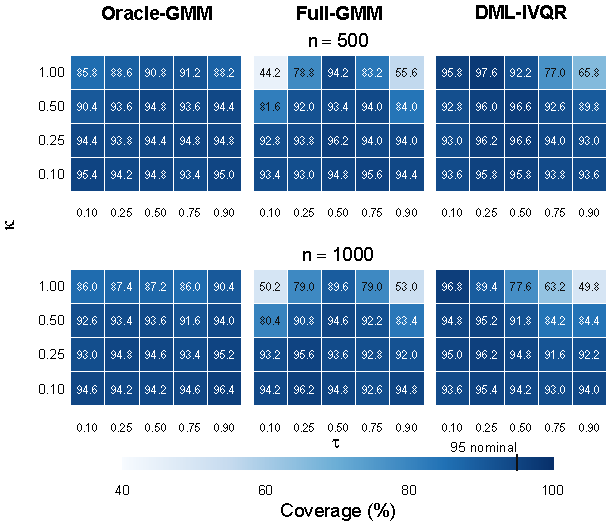
\includegraphics[width=0.72\textwidth]{figures/generated/coverage_heatmap.pdf}
  \caption{Empirical coverage across simulation designs.}
  \label{fig:coverage-heatmap}
  \begin{figurenotes}
    Nominal coverage is 95\%; each cell uses 500 complete replications. Coverage is the fraction of tests accepting the true parameter, evaluated directly at that parameter rather than reconstructed from grid membership. Panel columns identify estimators; panel rows show $n=500$ and $n=1000$. Within each panel, columns show quantiles $\tau$ and rows show relevance $\kappa$, declining from 1.00 to 0.10. Annotations and the common colour scale report percentages. Darker shading indicates higher coverage, not necessarily better calibration.
  \end{figurenotes}
\end{figure}


Increasing the sample size can improve point accuracy without improving calibration. At $\kappa=1$, DML coverage falls from $0.976$ to $0.894$ between $n=500$ and $n=1000$ at $\tau=0.25$, from $0.922$ to $0.776$ at $\tau=0.50$, from $0.770$ to $0.632$ at $\tau=0.75$, and from $0.658$ to $0.498$ at $\tau=0.90$. These changes equal $-8.2$, $-14.6$, $-13.8$, and $-16.0$ percentage points. Section~\ref{sec:results-point-accuracy} found lower RMSE at $n=1000$ in all 60 matched comparisons, so lower observed RMSE of the grid minimiser does not imply that the candidate-specific test has size closer to its nominal level.

Coverage tends to move toward $0.95$ as relevance weakens, but not monotonically in every cell. Averaged over estimators, quantiles, and sample sizes, coverage rises from $0.798$ at $\kappa=1$ to $0.912$, $0.941$, and $0.944$ as $\kappa$ falls. Only 15 of the 30 estimator--sample-size--quantile sequences are nondecreasing at every step. For example, DML coverage at $n=1000$ and $\tau=0.10$ is $0.968$, $0.948$, $0.950$, and $0.936$ across declining $\kappa$, while Full-GMM coverage at $n=500$ and $\tau=0.25$ is $0.788$, $0.920$, $0.938$, and $0.930$. These reversals are generally small compared with the strong-relevance distortions. More importantly, movement toward nominal coverage under weak relevance can result from rejecting candidate values less often overall.

Each rate is based on $R=500$ replications. Its Monte Carlo standard error is
\[
\operatorname{MCSE}(\widehat p)
=
\sqrt{\frac{\widehat p(1-\widehat p)}{R}}.
\]
The maximum MCSE is approximately $0.022$ and the MCSE at $0.95$ is approximately $0.010$. Appendix~\ref{app:coverage-forensic-audit} strengthens this cell-by-cell uncertainty check. Across 60,000 valid direct-at-truth evaluations, 53 pointwise two-sided 95\% Wilson intervals lie wholly below $0.95$, one lies wholly above it, and 66 contain it. No truth statistic is missing or nonfinite. The intervals use integer acceptance counts without a continuity correction; they are pointwise Monte Carlo intervals, not simultaneous or multiplicity-adjusted tests. An individual rate's MCSE is not used as the standard error of a difference between correlated simulation results.

The audit rules out missing-value handling, nonfinite truth statistics, and reconstruction from rounded grid confidence sets as explanations for the observed undercoverage. It does not isolate a cause among finite-sample approximation error, features of the preserved implementation, or failure of the idealised regularity conditions for the asymptotic chi-square reference law in this DGP. Strong-relevance undercoverage also shows that weak relevance alone cannot explain the distortions. Coverage records retention of the truth; it does not record how readily false candidates are excluded. The next two sections therefore examine power and accepted-set informativeness before interpreting near-nominal coverage under weak relevance.

\subsection{Power Against False Candidate Values}
\label{sec:results-power}

Figure~\ref{fig:power-median-combined} reports rejection probabilities at $\tau=0.50$ for candidate values $a_{\Delta}(\tau)=\alpha_0(\tau)+\Delta$. At $\Delta=0$, the candidate is true and rejection probability is empirical size; at each of the six nonzero deviations, it is empirical power against that specified false candidate. The data-generating parameter remains fixed throughout. The plotted probabilities use the same nominal 5\% chi-square cutoff and are not adjusted for differences in empirical size.

\begin{figure}[!htbp]
  \centering
  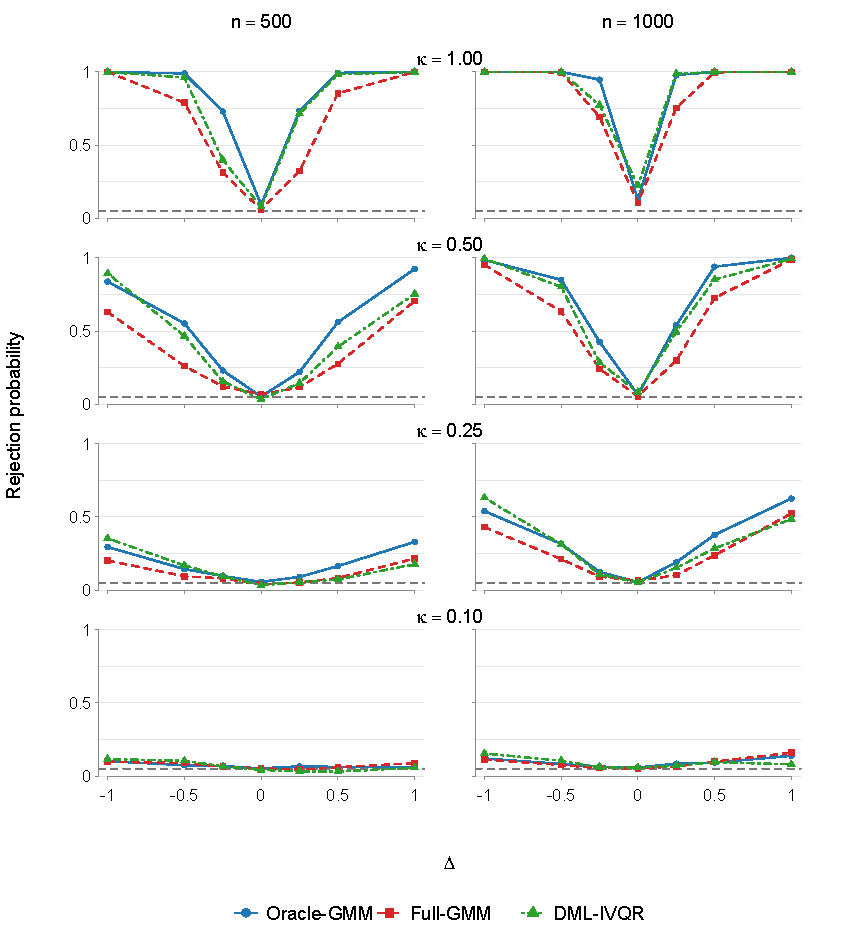
\includegraphics[width=\linewidth]{figures/generated/power_median_combined.pdf}
  \caption{Empirical power at the median.}
  \label{fig:power-median-combined}
  \begin{figurenotes}
    The median benchmark is $\tau=0.50$. Columns show $n=500$ and $n=1000$; rows show $\kappa=1.00,0.50,0.25,0.10$. The horizontal axis is $\Delta=a-\alpha_0(0.50)$, the saved deviation of the tested candidate from truth. Each point uses 500 complete replications and the same nominal 5\% chi-square cutoff; dashed horizontal lines mark 0.05. Rejection at truth is evaluated directly. At $\Delta=0$, rejection probability measures empirical size; at nonzero deviations, it measures power. These rejection probabilities are not size-adjusted. Straight segments are visual guides between evaluated points.
  \end{figurenotes}
\end{figure}


At $n=1000$ and $\Delta=-0.50$, Oracle power falls from $1.000$ through $0.850$ and $0.316$ to $0.082$ as $\kappa$ declines, while DML falls from $1.000$ through $0.802$ and $0.312$ to $0.104$. Full-GMM likewise falls from $0.998$ to $0.076$ between the strongest and weakest settings. For $\Delta=0.50$ at $\kappa=0.25$, power is $0.378$, $0.238$, and $0.286$ for Oracle, Full, and DML, before falling to approximately one tenth for all three at $\kappa=0.10$. The deterioration is therefore already substantial at intermediate relevance, and false effects separated from truth by one half become difficult to exclude in the weakest setting.

Increasing $n$ usually raises power where usable signal remains. At $\kappa=0.50$, Oracle power at $\Delta=-0.50$ rises from $0.552$ to $0.850$, Full from $0.260$ to $0.634$, and DML from $0.466$ to $0.802$ between $n=500$ and $n=1000$. At $\Delta=0.50$, the corresponding changes are $0.560$ to $0.940$, $0.276$ to $0.726$, and $0.392$ to $0.852$. At $\kappa=0.10$, improvements are much smaller and not uniform: Full power at $\Delta=-0.50$ falls from $0.088$ to $0.076$, while DML remains $0.104$; at $\Delta=0.50$, DML rises from $0.030$ to $0.094$. Across all five quantiles and six nonzero deviations, $n=1000$ has higher rejection probability in 305 of 360 matched cells, the same probability in 25, and a lower probability in 30.

The null points clarify why raw power cannot be used as an efficiency ranking. At $n=1000$ and $\kappa=1$, median empirical size is $0.128$ for Oracle, $0.104$ for Full, and $0.224$ for DML, compared with $0.092$, $0.058$, and $0.078$ at $n=500$. DML's strong-relevance rejection of false candidates therefore coexists with the size distortion documented in Section~\ref{sec:results-coverage}. At $n=1000$ and $\kappa=0.10$, empirical sizes are $0.058$, $0.052$, and $0.058$, while power at $\Delta=-0.50$ is only $0.082$, $0.076$, and $0.104$. Rejection of this false candidate is then close to rejection at truth, indicating little discrimination despite approximately nominal size.

The median pattern broadly generalises, but it is not universally monotone. Across all quantiles, sample sizes, estimators, and nonzero deviations, power is nonincreasing as $\kappa$ falls in 162 of 180 sequences. The 18 exceptions are mostly small reversals when rejection is already close to empirical size. Signed differences also occur: for DML at $\tau=0.50$, $n=500$, and $\kappa=0.25$, power is $0.168$ at $\Delta=-0.50$ but $0.072$ at $\Delta=0.50$. Figure~\ref{fig:power-median-combined} displays only $\tau=0.50$, so these full-result counts support generalisation without implying that every quantile follows the plotted paths. The design does not isolate the source of signed asymmetry, and asymmetry in power is not by itself evidence of point-estimation bias.

\FloatBarrier

\subsection{Confidence-Set Informativeness}
\label{sec:results-informativeness}

Figure~\ref{fig:accepted-measure-main} reports the median grid-based accepted-set measure within $A_0=[-1,3]$. The measure increases strictly at every step as $\kappa$ falls in all 30 estimator--sample-size--quantile sequences. At $n=1000$ and $\tau=0.50$, Oracle, Full, and DML medians rise from $0.200$, $0.400$, and $0.300$ at $\kappa=1$ to $3.900$, $3.800$, and $3.900$ at $\kappa=0.10$. Thus declining relevance causes progressively more of the maintained domain to survive test inversion, even when coverage moves closer to $0.95$.

\begin{figure}[!htbp]
  \centering
  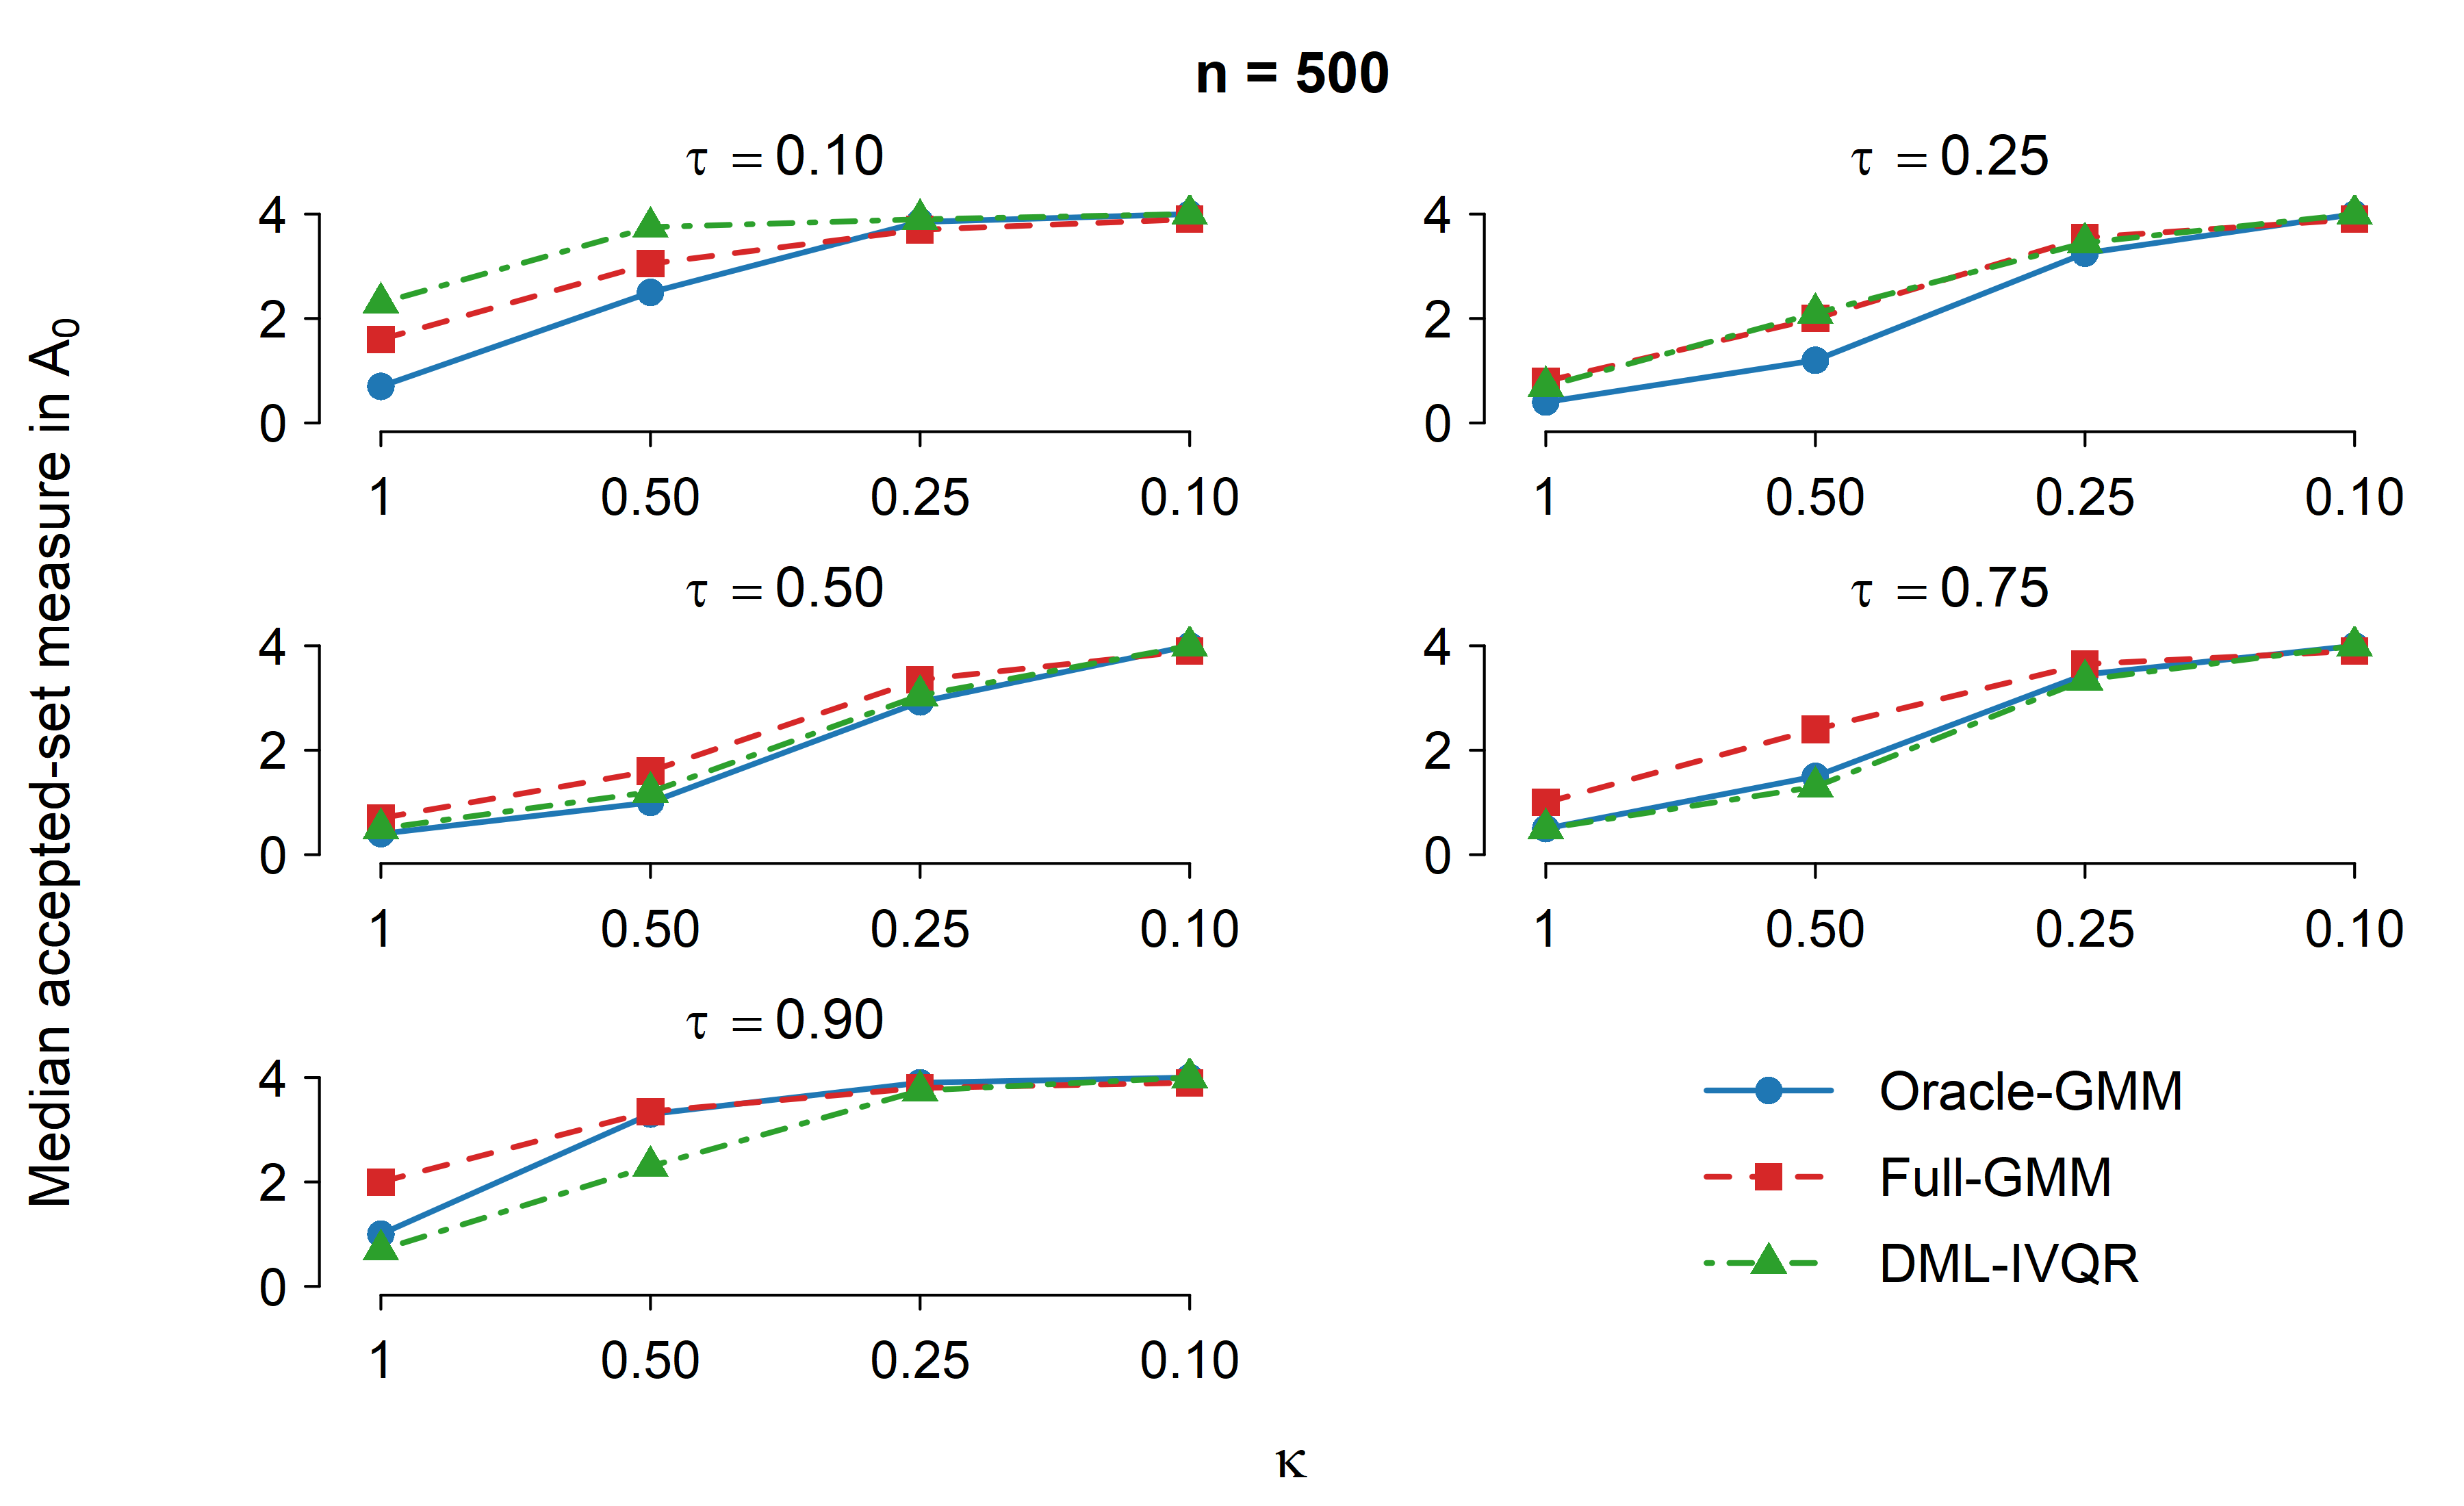
\includegraphics[width=\linewidth]{figures/generated/accepted_measure_n500.png}
  \par\medskip
  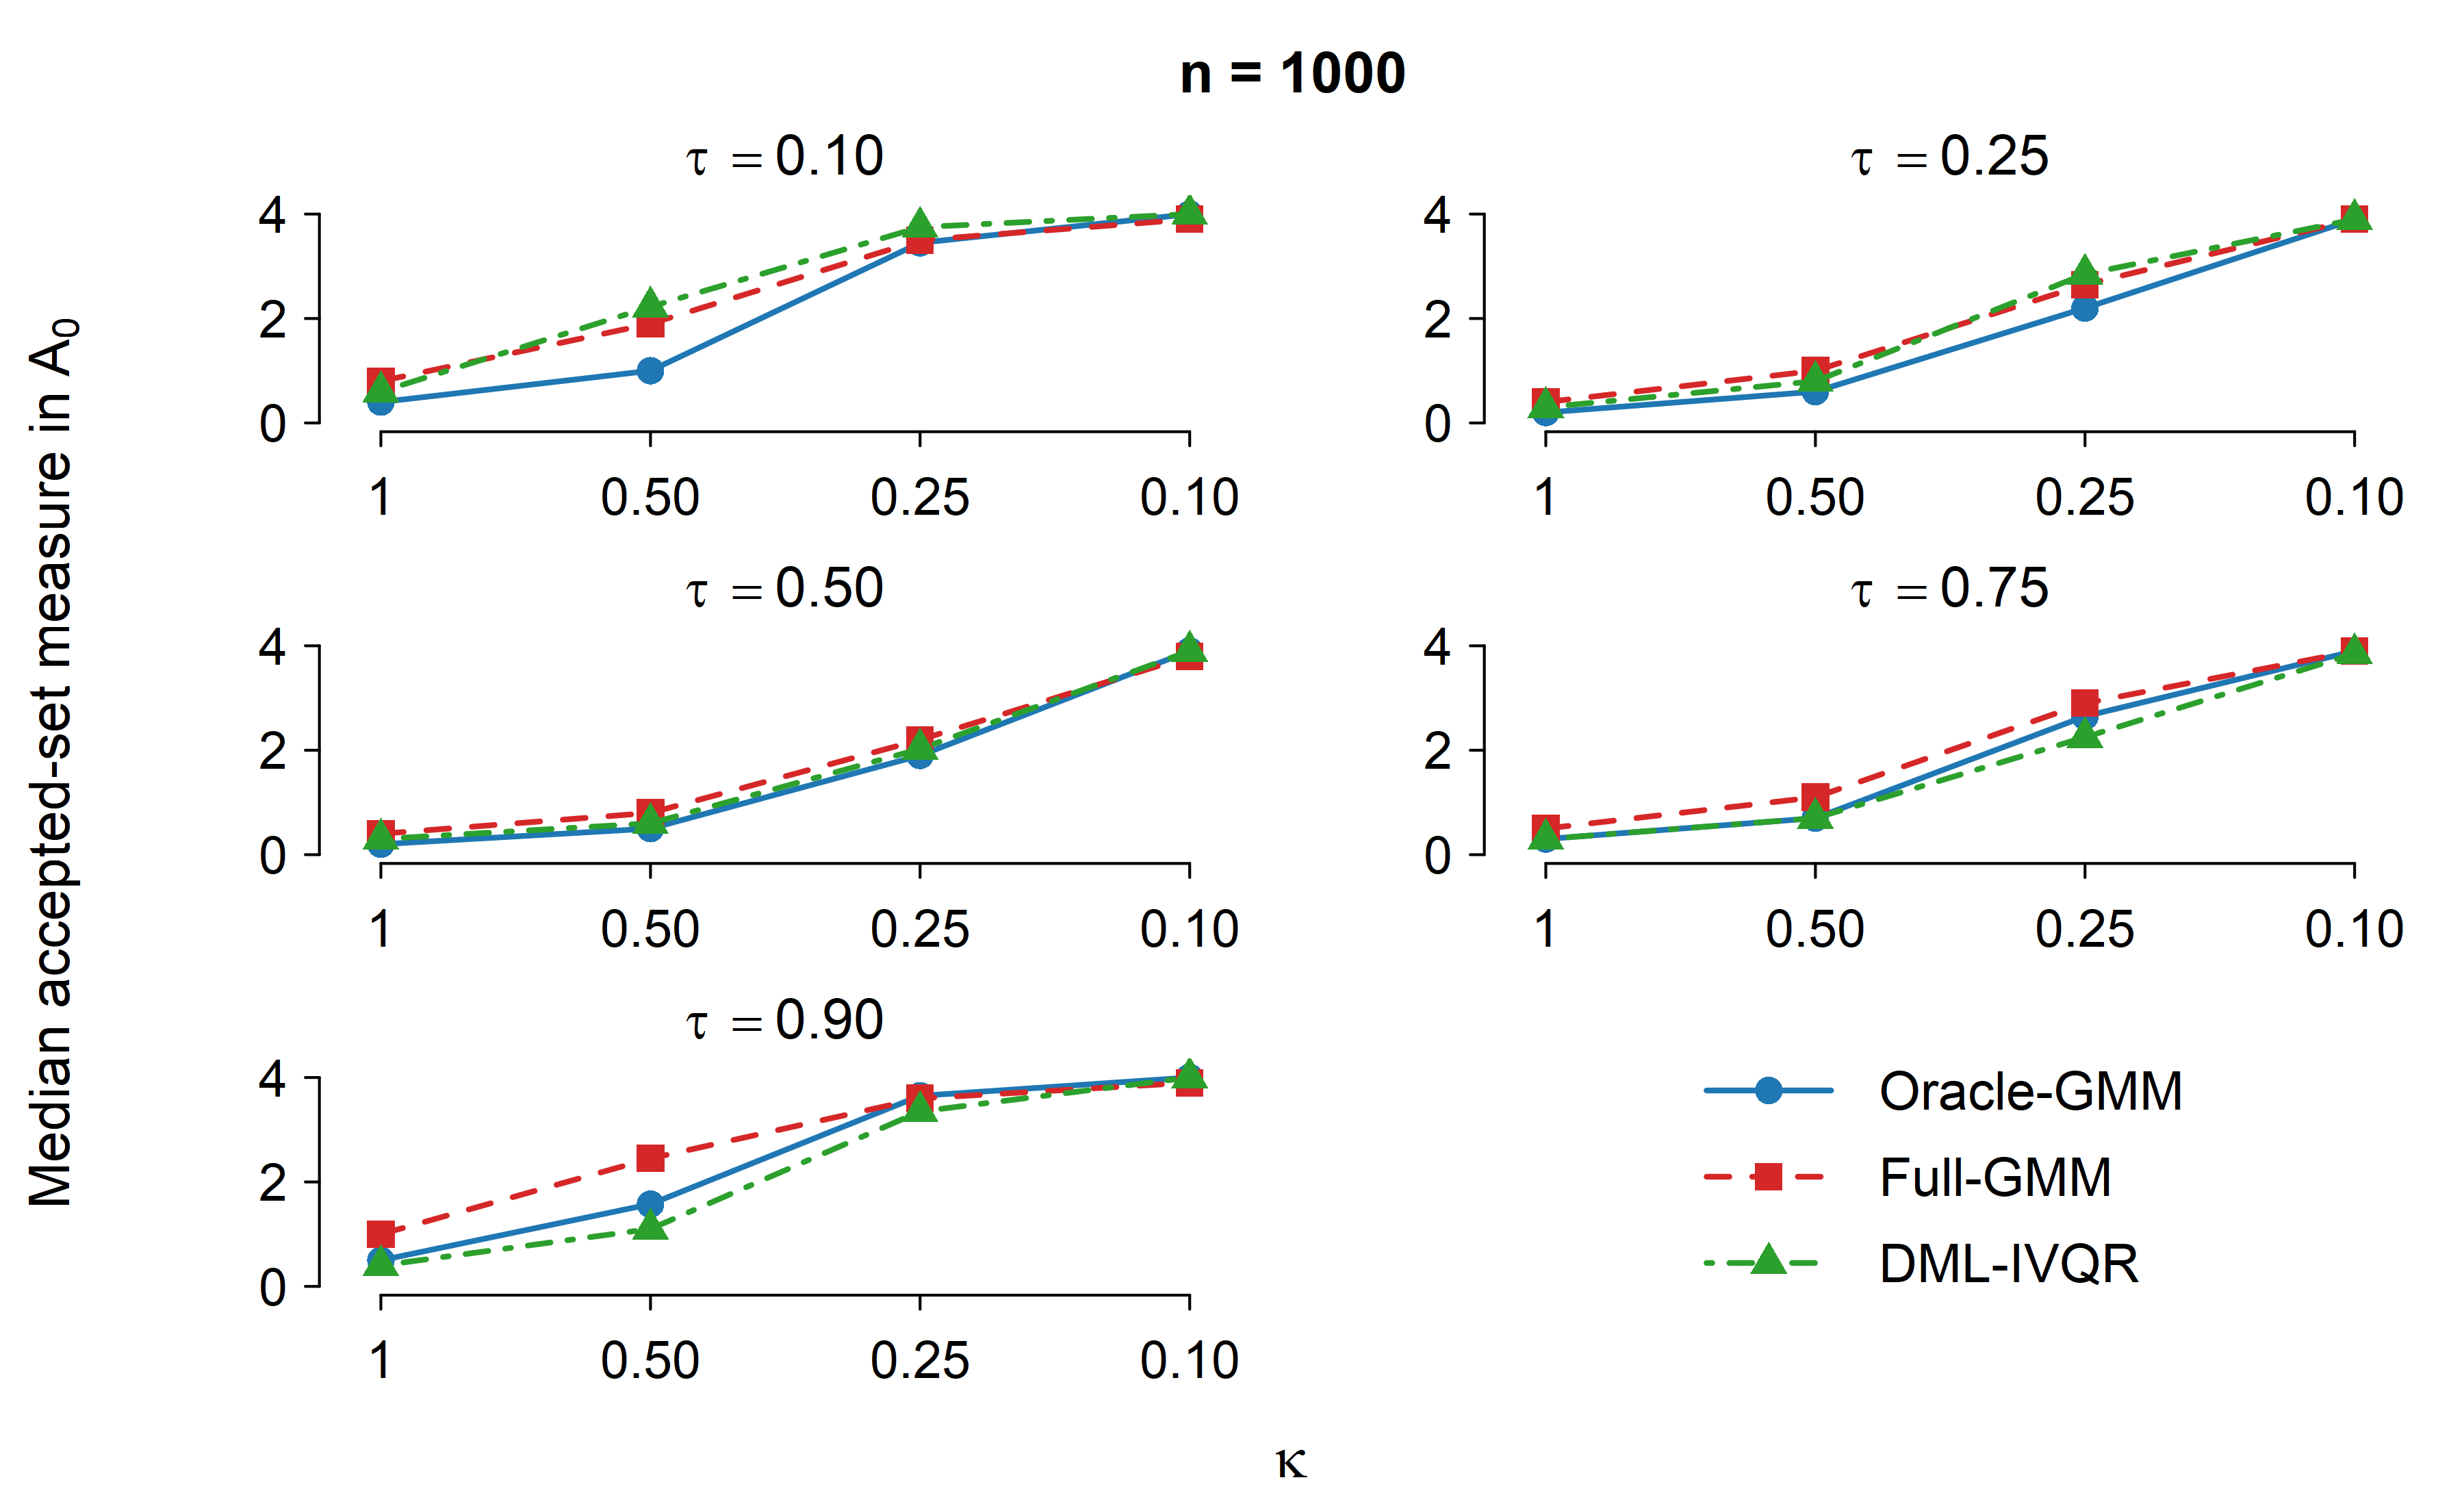
\includegraphics[width=\linewidth]{figures/generated/accepted_measure_n1000.png}
  \caption{Grid-based accepted-set measure within the primary computational domain $A_0=[-1,3]$.}
  \label{fig:accepted-measure-main}

\begin{figurenotes}
Panels show $n=500$ and $n=1000$, using 500 replications per cell. Curves identify Oracle-GMM, Full-GMM, and DML-IVQR; quantile panels show $\tau$. Plotted values are replication medians of the trapezoidal binary-grid-acceptance measure at each $\kappa$. The maximum is four, the width of $A_0$; this is not unrestricted confidence-region length. Lines join evaluated relevance settings as visual guides.
\end{figurenotes}
\end{figure}


Quantile and estimator differences are visible before the weakest setting. At $n=1000$ and $\kappa=0.50$, DML's median measure ranges from $0.600$ at $\tau=0.50$ to $2.225$ at $\tau=0.10$, while Full ranges from $0.800$ to $2.450$ across the five quantiles. Increasing the sample size narrows the median accepted measure in 52 of 60 matched cells and leaves it unchanged in eight; it never widens it. For example, DML at $\tau=0.50$ and $\kappa=0.25$ falls from $3.050$ to $2.025$, whereas at $\kappa=0.10$ it falls only from $4.000$ to $3.900$. More observations improve localisation, but do not overcome the weakest relevance setting at these sample sizes.

The DML sequence at $n=1000$ and $\tau=0.50$ connects the four inferential summaries. At $\kappa=1$, coverage is $0.776$, the median accepted measure is $0.300$, the full-grid acceptance rate is $0.000$, and power at $\Delta=0.50$ is $1.000$. At $\kappa=0.25$, the corresponding values are $0.948$, $2.025$, $0.040$, and $0.286$. At $\kappa=0.10$, coverage remains near nominal at $0.942$, but the median measure is $3.900$, full-grid acceptance is $0.428$, and power at $\Delta=0.50$ is $0.094$. Truth retention, the amount of the grid retained, acceptance of the entire grid, and rejection of a particular false value therefore answer different questions.

The measure cannot exceed four because it integrates grid acceptance only over $A_0=[-1,3]$. Similar values near four do not imply equivalent unrestricted confidence regions: the calculation does not examine candidates outside $A_0$, and distinct acceptance patterns can produce similar totals. Supplementary Figure~\ref{fig:appendix_full_domain_acceptance} records the frequency with which all 41 evaluated points are accepted. That event does not establish acceptance at every intermediate real value or anywhere outside $A_0$. Coverage is also a separate direct evaluation at truth. For DML, fresh pivotal draws mean that direct-truth coverage and stored-profile acceptance need not coincide even when truth is numerically a grid point.

Appendix~\ref{app:numerical-domain-diagnostics} examines wider domains in a separate diagnostic with $n=1000$, 100 replications, all five quantiles and estimators, $\kappa\in\{1,0.25,0.10\}$, and step $0.1$ on $A_0=[-1,3]$, $A_1=[-3,5]$, and $A_2=[-5,7]$. At $\tau=0.50$ and $\kappa=1$, median DML measure remains $0.300$ on all three domains and $A_2$ boundary acceptance is zero. At $\kappa=0.25$, it grows from $1.950$ to $2.500$ and $3.025$, with $A_2$ boundary acceptance $0.500$. At $\kappa=0.10$, it grows from $3.900$ to $7.500$ and $10.325$, and the $A_2$ boundary is accepted in $0.960$ of usable profiles. Oracle and Full display the same broad weak-relevance pattern, with $A_2$ median measures $11.300$ and $11.450$ and boundary rates $0.830$ and $0.850$ in the corresponding cell.

These domain-expansion values come from a diagnostic run with 100 replications, not the main 500-replication experiment. They show near-stability within the investigated domains under strong relevance and continued failure to localise at intermediate and weak relevance. The diagnostic ends at $A_2$ and does not search the real line. Failure to localise over these domains is evidence of limited numerical informativeness, not proof of global unboundedness or non-identification.

\FloatBarrier
